\chapter{Controleren op kwaliteitsgebreken}\label{sec:kwaliteitsgebrek}
Waar in hoofdstuk \ref{sec:consistentie} objecten centraal stonden, doen we daar hier afstand van: we abstraheren de logische types voor klasses weg en concentreren ons in de plaats op \textit{ClassObject}, een logisch type dat een overeenkomstig object heeft voor alle klasses in het diagram. We gebruiken het diagram in figuur \ref{fig:diagram-voorbeeld} weer als begeleidend voorbeeld. In de volgende subsecties overlopen we hoe we de theorie die we gebruiken voor dit probleem opbouwen.

\section{Gebruikte logische types en predicaten}
Waar we in sectie \ref{sec:hierarchies} het logisch type \textit{ClassObject} en het predicaat \textit{IsSupertypeOf/2} afwezen, behouden we ze hier en berekenen we de transitieve sluiting van \textit{IsSupertypeOf/2} zoals beschreven in diezelfde sectie.

We gebruiken daar bijkomend de volgende nieuwe predicaten:

\begin{itemize}
	\item \textbf{\textit{BiAssoc(ClassObject,ClassObject)}}: drukt uit dat er een binaire associatie bestaat tussen de twee klasses.
	\item \textbf{\textit{BiAssocLow(ClassObject,ClassObject,ClassObject,nat)}}: voor \textit{BiAssocLow(x,y,x,n1)} geldt dat voor de binaire associatie tussen klasse \textit{x} en klasse \textit{y} de ondergrens voor de multipliciteit aan de \textit{x}-kant gelijk is aan \textit{n1}; een gelijkaardige interpretatie geldt voor \textit{BiAssocLow(x,y,y,n2)}.
	\item \textbf{\textit{BiAssocHigh(ClassObject,ClassObject,ClassObject,nat)}}: gelijkaardig aan \textit{BiAssocLow/4}, maar dan voor de bovengrens van de multipliciteit.
\end{itemize}

Deze predicaten worden ingevuld met een lijst van feiten die af te lezen zijn van het diagram. In hoofdstuk \ref{sec:rol-idp} wordt de logische theorie die het resultaat is van dit proces weergegeven.

\section{Kwaliteitsgebreken detecteren}
Er zijn drie kwaliteitsgebreken waarnaar wordt gezocht in de resulterende theorie:

\begin{itemize}
	\item \textbf{Many-to-many associaties}: Dit zijn associaties waar de bovengrens van de multipliciteiten aan beide kanten gelijk is aan $*$. Het voorkomen van een many-to-many associatie is doorgaans een teken dat er een klasse ontbreekt in het ontwerp. Het is dus van groot belang dat dit wordt opgespoord en opgelost.
	
	\item \textbf{Losstaande klasse}: Concreet is een losstaande klasse een klasse die geen associatie heeft met een andere klasse in het ontwerp. Zulk een klasse is nutteloos en moet ofwel verbonden worden met een andere klasse of verwijderd worden.
	
	\item \textbf{Overbodige associaties in een klassehi\"erarchie}\cite{Balaban2015}: Beschouw figuur \ref{fig:hierarchie}. Daar is te zien dat de grenzen van de multipliciteiten in de associatie \textit{Alice}---\textit{Charlie} strengere voorwaarden opleggen dan die van de associatie \textit{Bob}---\textit{David}, en dat daarom de associatie \textit{Bob}---\textit{David} overbodig is. Om de verstaanbaarheid van het diagram te verbeteren, wordt die associatie best verwijderd.
\end{itemize}

We defini\"eren deze respectievelijke gebreken in de logische theorie door middel van de volgende logische zinnen:

\begin{align}
	\nonumber \forall{x}[ClassObject]\forall{y}[ClassObject](ManyToMany(x,y) \Leftrightarrow BiAssoc(x,y) \land \\ \lnot\exists{z}[nat](BiAssocHigh(x,y,x,z)) \land \lnot\exists{z}[nat](BiAssocHigh(x,y,y,z))).\label{form:manytomany}
\end{align}

\begin{align}
	\nonumber \forall{x}[ClassObject](LooseClass(x) \Leftrightarrow \lnot(\exists{y}[ClassObject](\lnot(x = y) \land (BiAssoc(x,y) \\ \lor \exists{s}[ClassObject]\exists{y}[ClassObject](IsSupertypeOf(s,x) \land BiAssoc(s,y)))))).\label{form:loose}
\end{align}

\begin{figure}
	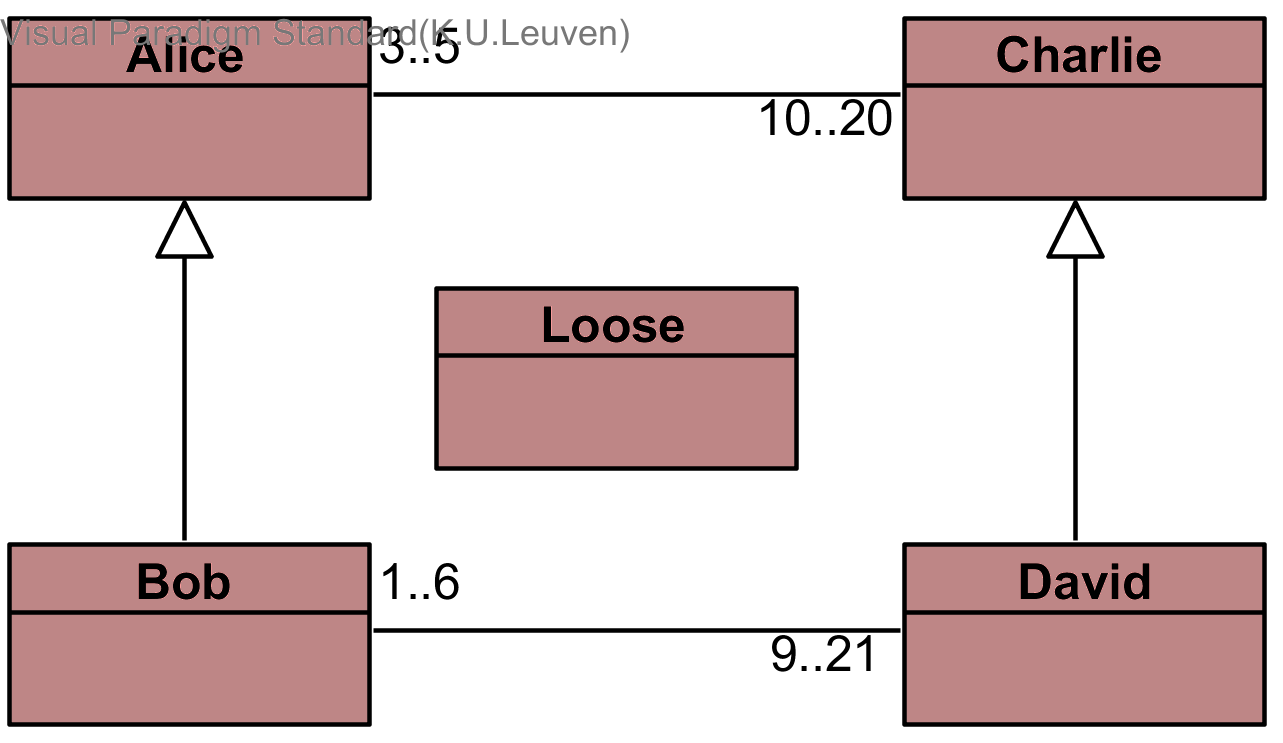
\includegraphics{chap-kwaliteitsgebrek/hierarchy.png}
	\caption{Voorbeeld van meer permissieve multipliciteiten in een klassehi\"erarchie en van een losstaande klasse (zijnde \textit{Loose})}
	\label{fig:hierarchie}
\end{figure}

Zin \ref{form:manytomany} controleert of voor beide rollen van een associatie geldt dat bovengrens * is. Zin \ref{form:loose} controleert of klasse \textit{x} rechtstreeks geassocieerd is met een andere klasse, en zoniet, of klasse \textit{x} een subklasse is van een andere klasse en of die superklasse geassocieerd is met nog een andere klasse.

De zin die overbodige associaties opspoort is te uitgebreid om op een duidelijke manier in deze tekst neer te zetten. Hij is terug te vinden in bijlage \ref{app:kwaliteitsgebrek}.
Deze zin onderscheidt drie gevallen:

\begin{itemize}
	\item Klasse \textit{x} en klasse \textit{y} zijn geassocieerd. Er bestaat een klasse \textit{Sx} die een superklasse is van \textit{x} en ook geassocieerd is met \textit{y}. De associatie \textit{x}---\textit{y} heeft aan het uiteinde \textit{x} ofwel een lagere ondergrens dan de associatie \textit{Sx}---\textit{y} aan uiteinde \textit{Sx} of een grotere bovengrens.
	\item Klasse \textit{x} en klasse \textit{y} zijn geassocieerd. Er bestaat een klasse \textit{Sy} die een superklasse is van \textit{y} en ook geassocieerd is met \textit{x}. De associatie \textit{x}---\textit{y} heeft aan het uiteinde \textit{x} ofwel een lagere ondergrens dan de associatie \textit{x}---\textit{Sy} aan uiteinde \textit{x} of een grotere bovengrens.
	\item Klasse \textit{x} en klasse \textit{y} zijn geassocieerd. Er bestaat de klasse \textit{Sx} die een superklasse is van \textit{x} en een klasse \textit{Sy} die een superklasse is van \textit{y}. De associatie \textit{x}---\textit{y} heeft aan het uiteinde \textit{x} ofwel een lagere ondergrens dan de associatie \textit{Sx}---\textit{Sy} aan uiteinde \textit{Sx} of een grotere bovengrens.
\end{itemize}

In hoofdstuk \ref{sec:rol-idp} wordt uitgelegd hoe deze theorie wordt gebruik om kwaliteitsgebreken te vinden.